\documentclass[a4paper]{article}
\usepackage[a4paper,left=2.5cm,right=2cm,top=2.5cm,bottom=2.5cm]{geometry}
\input{preamble.tex}

\title{Reinforcement learning}

\begin{document}
    \maketitle
    \tableofcontents
    \newpage
    % start lectures
    \lesson{1}{monday 15 jan 2023 10:15}{Introduction}

\section{Introduction to the course}



    \section{Markov Decision process}
This lecture will explain the concepts of Markov decision process, MDP's, the Bellman equation and optimal policy

\subsection*{Recap}
For a state to have \textbf{Markov property} means that the state contains all the information that is useful to predict the future. In other words, we don't need the previous states to predict the future, the useful information is stored in the current state. A \textbf{Policy}: $\pi$(a|s) choosing an action a when we are in state s, can be deterministic or stochastic. The \textbf{prediction} gives the future cumulative reward following a policy. We want to find the policy that maximize the cumulative future reward by \textbf{control}. 

\subsection*{Markov decision process}
If we begin with assuming that $\mathcal{S}, \mathcal{A} $ and $\mathcal{R}$ have finite numbers of elements then the \textbf{translation probabilities} are given by:

	\begin{equation}
		p(^{\prime},r |s,a) = \text{Pr}\{S_{t+1} = s^{\prime}, R_{t+1} = r | S_t = s, A_t = a \}
	\end{equation}

The Markov property determines the \textbf{dynamics} of the environment, the probability of transitioning to a new state depends only on the current state and action. The \textbf{state transitions}:

	\begin{equation}
		p(s^{\prime} | s,a) = \sum_{r \in \mathcal{R}} p(s^{\prime},r |s,a) =
	\end{equation}

With the \textbf{expected reward }

	\begin{equation}
		r(s,a) = \mathbb{E} [ R_{r+1} | S_t = s, A_t = a ] =  \sum_{r \in \mathcal{R}}^{} \sum_{s^{\prime \in \mathcal{S}}}^{} r p(s^{\prime},r | s,a)  
	\end{equation}

\subsection*{Episodic vs continuing tasks}
\begin{itemize}
	\item \textbf{Episodic tasks}
	\begin{itemize}
		\item Has terminating states and the task end in finite time.
		\item When reaching the terminating state the episode stops.
		\item If you reach the terminating state you will stay there forever, receiving no future rewards.
	\end{itemize}
	\item \textbf{Continuing tasks}
	\begin{itemize}
		\item Often not a clear way to divide the task into independent episodes.
		\item No state were the task is done
		\item Must take into account infinitely many future rewards.
	\end{itemize}
\end{itemize}


\subsection*{The return}
In a given state we want to maximize the future reward we can receive: $R_{t+1},R_{t+2, ...}$. To make it possible to have non finite number of rewards we introduce the \textbf{discounted reward}

	\begin{wbox}{The discounted reward}
		\begin{equation}
			G_t = R_{t+1} R_{t+1} + \gamma R_{t+2} + \gamma^{2} R_{t+3} + \ldots = \sum_{k=0}^{\infty} \gamma^{k}R_{t+k+1}, \text{where } 0 < \gamma \le 1
		\end{equation}
	\end{wbox}

since we put $\gamma \le 1$ we put less value on future rewards, $\gamma = 0.5 \Rightarrow \gamma^{10} = 0.001, \gamma = 0.9 \Rightarrow \gamma^{10} = 0.35$.

And if $\gamma < 1$ we make sure that $R_t < \overline{R}$ for all t, and then $G_t$ is bounded:

	\begin{equation}
		\sum_{k=0}^{\infty} \gamma^{k}R_{t+k+1} \le \overline{R}\sum_{k=0}^{\infty} \gamma^{k} = \frac{1} {1-\gamma} \overline{R}
	\end{equation}


If we know that the task ends after a finite number of steps we can get away with using non-discounted returns where $\gamma = 1$

\subsection*{The state value function}
The state-value function estimates the expected long term rewards the agent will recieve starting from a specific state and following a given policy. Since $S_t$ and $R_t$ are random variables, the return is therefore also a random variable:

	\begin{equation}
		G_t = R_{t+1} + \gamma R_{t+2} + \ldots
	\nonumber
	\end{equation}

We must therefore consider the expected return:

	\begin{wbox}{The state-value function}
	The state-value function $v_\pi (s)$ of a MDP is the expected return starting from the state s and then following the policy $\pi$:

		\begin{equation}
			v_\pi (s) = \mathbb{E}[G_t | S_t = s]
		\end{equation}
	\end{wbox}

The prediction of cumulative reward is computed with $v_\pi(s)$



\subsection*{The action-value function}
Another important value function is the \textbf{action-value function} that estimates the expected long-term reward an agent will receive starting from a specific state, taking a specific action and following a given policy.

	\begin{wbox}{The action-value function}
	The action-value function $q_\pi(s,a)$ is the exptected return starting from s, taking action a, and \textbf{then} following a policy $\pi$
		\begin{equation}
			q_\pi (s,a) = \mathbb{E}[G_t | S_t = s, A_t = a]
		\end{equation}
	\end{wbox}

This function is also often called the Q-function. 

\subsection*{Bellman equations}
Looking at the reward we can note that:

	\begin{equation}
		G_t = R_{t+1} + \gamma R_{t+2} + \gamma^{2} R_{t+3} + ... = R_{t+1} + \gamma G_{t+1}
	\end{equation}

Hence, the value function satisfies to following equation:

	\begin{equation}
	\begin{aligned}
		v_\pi(s) = \mathbb{E}_\pi [G_t | S_t = s]\\
		= \mathbb{E}_\pi [R_{t+1} + \gamma G_{t+1} | S_t = s] \\
		= \mathbb{E}_\pi [R_{t+1} + \gamma v_\pi(S_{t+1}) | S_t =s ]
	\end{aligned}
	\end{equation}

The value of s is the expected immediate reward plus the discounted expected vlue of the next state. In the same way is action-value function: 

	\begin{equation}
		q_\pi (s,a) = \mathbb{E} [R_{t+1} + \gamma q_\pi(S_{t+1}, A_{t+1} | S_t = s, A_t = a)]
	\end{equation}
	

\begin{wbox}{}
	\begin{equation}
	\begin{aligned}
		v_\pi(s) = \mathbb{E}_\pi [R_{t+1} + \gamma v_\pi(S_{t+1}) | S_t =s ]\\
		q_\pi (s,a) = \mathbb{E} [R_{t+1} + \gamma q_\pi(S_{t+1}, A_{t+1} | S_t = s, A_t = a)] 
	\end{aligned}
	\end{equation}
\end{wbox}

\subsection*{The expectation}
The state-value of a state s, is the expected action-value:

	\begin{equation}
		v_\pi(s)= \sum_{a}^{} \pi(a |s) q_\pi(s,a)
	\end{equation}

So for a deterministic policy a = $\pi(s)$ we get $v_\pi(s,\pi(s))$. And given s and a, the immediate reward r and the next state $s^{\prime}$ has probability $p(s^{\prime}, r |s,a)$ so that:

	\begin{equation}
		q_\pi (s,a) = \sum_{r, s^{\prime}}^{} p(s^{\prime},r | s,a) (r + \gamma v_\pi(s^{\prime})) 		
	\end{equation} 


	\begin{wbox}{The Bellman equation for $v_\pi$ and $q_\pi$}
		\begin{equation}
		\begin{aligned}
			v_\pi = \sum_{a}^{} \pi(a |s)q_\pi(s,a) = \sum_{a}^{} \pi(a,s)\sum_{r, s^{\prime}}^{} p(s^{\prime}, r | s, a)[r + \gamma v_\pi(s^{\prime})] \\
			q_\pi(s,a) = \sum_{r, s^{\prime}}^{} p(s^{\prime},r |s,a) [r + \gamma \sum_{a^{\prime}}^{} \pi(a^{\prime} |s^{\prime})q_\pi(s^{\prime},a^{\prime})]
		\end{aligned} 
		\end{equation}
	\end{wbox}
	








    %!TEX root = master.tex

\section{Feed forward neural networks: Backpropagation}
This lecture will cover how backpropagation works, how to compute the derivatives and some implementation. 

\subsection*{Stepsize}
Stepsize also know as the learning rate controls how large steps we take and greatly affects the training of our model. Using a to small stepsize will cause the convergence to be very slow, it can also be that we get stuck in a local minimum. Using a to big learning rate/stepsize will cause overshooting, bouncing around the minumum but never get there. Or in the worse case it can cause divergence. 



\subsection*{Neural network - construction}
An artificial neural network is a sequential construction of several generalized linear regression models. It consists of \textbf{Inputs} (1, $x_1, x_2, \ldots, x_p$), \textbf{Hidden units} (1, $q_1,q_2,\ldots, q_U$) and an output $\hat{y}$

	\begin{equation}
	\begin{aligned}
		q_1 = h(b^{(1)}_1 + \sum_{j=1}^{p}W^{(1)}_{1j}x_j) \\
		q_2 = h(b^{(1)}_2 + \sum_{j=1}^{p}W^{(1)}_{2j}x_j) \\
		\vdots \quad \quad \quad \quad \vdots \\
		q_U = h(b^{(1)}_U + \sum_{j=1}^{p}W^{(1)}_{Uj}x_j)
	\end{aligned}
	\end{equation}

	\begin{equation}
		\hat{y} = b^{(2)} + \sum_{i=1}^{U}W^{(2)}_iq_i
	\end{equation}


In vector representation:

	\begin{equation}
	\begin{aligned}
		W^{1} = \begin{bmatrix} W^{(1)}_{11} & \ldots& W^{(1)}_{1p} \\ \vdots& & \vdots \\ W^{(1)}_{U1} & \ldots& W^{(1)}_{Up}  \end{bmatrix} , b^{(1)} = \begin{bmatrix} b^{(1)}_1 \\ \vdots \\ b^{(1)}_U \end{bmatrix}, q = \begin{bmatrix} q_1 \\ \vdots \\ q_U \end{bmatrix} \\
		 b^{(2)} = \begin{bmatrix} b^{2} \end{bmatrix}, W^{(2)} = \begin{bmatrix} W^{(2)}_1 \ldots W^{(2)}_U \end{bmatrix} \\
		 \hat{y} = W^{(2)}q + b^{2} ,
	\end{aligned}
	\end{equation}

\subsection*{Deep neural network}
A deep network with several layers will learn better but needs more training. A deep neural network with $L$ can be written like this: 

	\begin{equation}
	\begin{aligned}
		q^{(0)} = \textbf{x} \\
		q^{\ell} = h(\textbf{W}^{(\ell)}q^{(\ell -1)}+\textbf{b}^{(\ell)}), \quad \ell = 1, \ldots, L-1 \\
		\hat{y} = \textbf{W}^{(L)}q^{(L-1)}+ \textbf{b}^{(L)}
	\end{aligned}
	\end{equation}

All the weight matrices and offset vectors in all of the layers are the parameters of the network:

	\begin{equation}
		\textbf{$\theta$} = \{\textbf{W}^{(1)},\textbf{b}^{(1)},\ldots, \textbf{W}^{(L)},\textbf{b}^{(L)}\}
	\end{equation}

These parameters constitutes the parametric model $\hat{y} = f(\textbf{x};\textbf{$\theta$})$ If the number L is large we call this a \emph{deep neural network}.

\subsection*{Unconstrained numerical optimization}
When training the neural network we are considering the following optimization problems: 

	\begin{equation}
		\hat{\textbf{$\theta$}} = \underset{\theta}{\arg \text{min }}J(\textbf{$\theta$}), \quad J(\textbf{$\theta$}) = \frac{1} {n}\sum_{i=1}^{n}L(\textbf{x}_i, \textbf{y}_i, \textbf{$\theta$}) 
	\end{equation}

The \emph{global objective function} or "cost" J is the average loss over the training set. The best solution that can be found will be $\hat{\textbf{$\theta$}}$ which is the global minimizer $(\hat{\textbf{$\theta$}}^{A})$. This global minimizer is often really hard to find and we therefore have to settle for some of the local minimizers $(\hat{\textbf{$\theta$}}^{A},\hat{\textbf{$\theta$}}^{B},\hat{\textbf{$\theta$}}^{C})$. 

\begin{example}{Example: Iterative solution (gradient descent)}
\begin{enumerate}
	\item Pick a $\theta_0$
	\item While (not converged)
		\begin{itemize}
			\item Update $\theta_{t+1} = \theta_t - \gamma \textbf{g}_t$
			\item Update t := t+1 
		\end{itemize}
\end{enumerate}
$\gamma \in \mathbb{R}^{+}$ is the step length or the learning rate.
\end{example}	


\subsection*{How to compute derivatives - Backpropagation}
For every step during the optimization we need to calculate the gradient:

	\begin{equation}
		\textbf{g}_t = \nabla_\theta J{\theta} = \frac{1} {n} \sum_{i=1}^{n}\nabla_\theta L_i(\textbf{x}_i,\textbf{y}_i, \theta)
	\end{equation}

But how do we compute these partial derivative? $\nabla_\theta L_j = (\frac{\partial L_j} {\partial w_1},\frac{\partial L_j} {\partial w_2}, \ldots )$

We using the chain rules and the fact that derivatives propagating backwards up through the net: $\frac{\partial L} {\partial \text{input}} = \frac{\partial L} {\partial \text{output}}\frac{\partial \text{output}} {\partial \text{input}}$. Using a computational graph often helps simplify the understanding and work.

\subsection*{Compute partial derivatives}
We need to calculate the gradient, which is a vector of partial derivatives of the Loss function with respect to the weights $\nabla_\theta L_j = (\frac{\partial L_j} {\partial w_1},\frac{\partial L_j} {\partial w_2}, \ldots )$. Here the Loss is given by a rather nasty looking expression involving weight, images and outputs:

	\begin{equation}
		L(\text{Net}(x_i,\theta) = L(s(W_3h(W_2h(W_1)))),y_i) 
	\end{equation}

Which is for a given set of images: $\{x_i\}$ and the correct output $\{y_i\}$, the variables are all our model parameters: weight and offsets. If we assuming in total m number of tunable parameters, then this is a function:

	\begin{equation}
		f : R^{m} \rightarrow R
	\end{equation}

The partial derivative of f at a point \textbf{a} = $(a_1, \ldots, a_j, \ldots,a_m)$ with respect to the j-th variable $x_j$ is the following expression:

	\begin{equation}
		\frac{\partial} {\partial x_j}f(\textbf{a}) =  \lim_{h \rightarrow 0} \frac{f(a_1,\ldots, a_j +h, \ldots, a_m) - f(a_1, \ldots, a_j, \ldots, a_m)} {h} 
	\end{equation}

This tells us how the function f change, as we move a little bit, the length $h$, along the dimension $j$. There are two ways to do this:

\begin{itemize}
	\item The \textbf{numerical gradient}: which is an approximation, slow to compute but easy to write.
	\item The \textbf{analytic gradient}: which is fast to compute and exact but quite error prone.
\end{itemize}

In practice we can derive the analytic gradient, check the implementation with a numerical gradient to see if it works. To derive the analytic gradients it is simply putting the chain rule to use. Since our function f is a composition of other functions f(g(h(...))) we compose the problem into smaller simpler problems:

	\begin{equation}
	\begin{aligned}
		f(x,y,z) = (x+y) * z \\
		f(q,z) = q * z \\
		q(x,y) = x + y \\
		q(x,y) = x + y \\
		\frac{\partial f} {\partial x} = \frac{\partial f} {\partial q} \frac{\partial q} {\partial x} 
	\end{aligned}
	\end{equation}

The gradient (propagating backwards on the input side) is the local gradient of the node multiplied multiplied with the gradient arriving to the node from the output side. If the node is connected to multiple output nodes, sum up the gradients of the different paths. When using ReLu activation only pass gradients to the positive outputs. With deep neural networks there are many values multiplied together and this can lead to problems with vanishing or exploding gradients. A ReLu that never turns on during the training, will never move (zero gradient) these are called "a dead ReLu".


\subsection*{Summary}

\begin{itemize}
	\item \textbf{Neural network (NN)}: A nonlinear \emph{parametric} model constructed by stacking several linear models with intermediate nonlinear activation functions.
	\item \textbf{Activation function}: A nonlinear scalar function applied to each output element of the linear models in a NN.
	\item \textbf{Gradient descent}: An iterative optimization algorithm where we at each iteration take a step proportional to the negative gradient.
	\item \textbf{Learning rate}: A scalar and tunable parameter which decide the length of each gradient step in gradient descent.
	\item \textbf{Back-propagation}: An efficient method that is based on the chain rule to compute the gradients.  
\end{itemize}







    \section{3D viewing and projection}
This lecture will cover rotation around arbritary axis, the "view" coordinate system, change of coordinate system, change of frame (change of coordinate system + translation), how to postion a camera and projections (orthogonal and perspective).

	\subsection*{Rotation around an arbitary axis}
	For rotation around an arbritary axis \textbf{v}, we need to find a matrix \textbf{M} that aligns (1,0,0) with \textbf{v}, then apply \textbf{M$^{-1}$} , apply rotation and \textbf{M} to the object. Here \textbf{M} is the change of coordinate system. But how do we find \textbf{M}?

	\subsection*{Change of coordinate system}
	The goal of change of coordinate system is to express a point with two different sets of basis vectors:
	
		\begin{equation}
			\textbf{P} = x \textbf{e}_1 + y\textbf{e}_2 = 
			x^{\prime} \textbf{f}_1 + y^{\prime}\textbf{f}_2
		\end{equation}
	If we assume to know the basis vectors of the new coordinate system \textbf{f}, in terms of the old coordinate system \textbf{e}.

		\begin{equation}
		\begin{aligned}
				\textbf{f}_1 = a \textbf{e}_1 + b \textbf{e}_2 \\ \textbf{f}_2 = c \textbf{e}_1 + d \textbf{e}_2 
		\end{aligned}
		\end{equation}
	Applying this gives us:

	\begin{equation}
	\textbf{P} = x \textbf{e}_1 + y\textbf{e}_2 = 
	x^{\prime} \textbf{f}_1 + y^{\prime}\textbf{f}_2 =
	x^{\prime}(a \textbf{e}_1 + b \textbf{e}_2) + y^{\prime}(c \textbf{e}_1 + d \textbf{e}_2)
	\end{equation}

	Coordinates in \textbf{f} transferred to \textbf{e}:

		\begin{equation}
			\begin{bmatrix} x \\ y \end{bmatrix} =
			\begin{bmatrix} a& c \\b& d \end{bmatrix}
			\begin{bmatrix} x^{\prime} \\ y^{\prime} \end{bmatrix} = \textbf{M} \begin{bmatrix} x^{\prime} \\ y^{\prime} \end{bmatrix}
		\end{equation}
	If we want coordinates in \textbf{e} transferred to \textbf{f}:

		\begin{equation}
			\begin{bmatrix} x^{\prime} \\ y^{\prime} \end{bmatrix} =
			\begin{bmatrix} a& c \\b& d \end{bmatrix}^{-1}
			\begin{bmatrix} x \\ y \end{bmatrix} = \textbf{M}^{-1} \begin{bmatrix} x \\ y \end{bmatrix}		
		\end{equation}
	\textbf{M} is a pure rotation matrix if and only if the basis are Ortho-Normal (ON)-bases. In that case is \textbf{M} orthogonal and $\textbf{M}^{-1}=\textbf{M}^{T}$. An orthogonal matrix is a matrix where the rows and columns are mutually orthogonal unit-length vectors \textcolor{red}{?}. Some properties of two orthogonal matrices are: the product is always orthogonal, always invertible and the inverse of an orthogonal matrix is equal to the \textbf{transpose} of the matrix. 

	\noindent How do we construct this ON basis if we only have one vector \textbf{v}
		\begin{equation}
		\begin{aligned}
			v_1 = \frac{\textbf{v}} {|\textbf{v}|} 	 \\
			v_2 = \frac{v_1 \times v^{\prime}} {|v_1 \times v^{\prime}|} \\
			v_3 = v_1 \times v_2 
		\end{aligned}
		\end{equation}
	How do we find a vector $v^{\prime}$ that is not parallel to $v_1$? We could just pick a random vector and check if the norm of the cross product is non zero. The problem with that is the risk of numerical error if the cross product is close to 0. A better way is to pick two orthogonal vectors \textbf{u}$_1$ (1,0,0) and \textbf{u}$_2$ (0,1,0). If $|\textbf{u}_1 \times \textbf{v}_1| > |\textbf{u}_2 \times \textbf{v}_1|$, set \textbf{v}$^\prime$ = \textbf{u}$_1$, otherwise \textbf{v}$^\prime$ = \textbf{u}$_2$.

	\noindent We now have rotation about an arbitrary axis \textbf{v}:

		\begin{itemize}
			\item Construct an \textbf{ON}-basis where \textbf{v}$_1$=\textbf{v} is the first basis vector, 
			\item Construct a corresponding "change of coordinates" matrix \textbf{M}, which align (1,0,0) with \textbf{v}
			\item Apply \textbf{M}$^{-1}$ to object (transfering coordinates to a coordinate system where \textbf{v} is aligned with (1,0,0))
			\item Rotate around (1,0,0)
			\item Apply \textbf{M} (transfers coordinates back to the original coordinate system)
		\end{itemize}

		\subsection*{Some coordinate systems}
		Here follows some examples of coordinate systems in the pipeline:

			\begin{equation}
				p^{\prime} = V_p * P * C * V_t * M * p			
			\end{equation}

		\noindent The \textbf{view transform} v$_t$ puts the observer at the origin and align x and y axes with the ones of the screen. Uses a right hand coordinate system so the z-axis is pointing backwards. This simplifies the clipping, light perspective and HSR (\textcolor{red}{?}). The view transformation is a so called change of frame, a change of origin + a change of coordinate system. This can be split into a translation and a change of coordinate system :

		\begin{equation}
		 	\begin{bmatrix} x^{\prime} \\ y^{\prime} \end{bmatrix}= 
		 	\textbf{M}^{-1}\textbf{T}(-P_0)\begin{bmatrix} x \\ y \end{bmatrix}	
		 \end{equation} 	
		
		\noindent glm::lookAt creates a viewing matrix that is derived from an eye point indicating the center of the scene and an UP vector. This build the 4x4 matrix for you but what is described above is what going on behind the scenes. 

		\noindent The \textbf{projection} p. Two types of projections: \textbf{Perspective} and \textbf{Orthographic} projection. In the orthographic projection is the "center of projection" at infinity and the projected points are along the direction of projection DOP. This projection is easy to implement since we only need to set z = 0. 
			\begin{equation}
		 		\begin{bmatrix} x^{\prime} \\ y^{\prime} \\z^{\prime} \\ 1 \end{bmatrix} = \begin{bmatrix} 1& 0& 0& 0\\ 
		 		                0& 1& 0& 0\\
		 		                0& 0& 0& 0\\
		 		                0& 0& 0& 1\end{bmatrix} \begin{bmatrix} x \\ y \\ z \\ 1 \end{bmatrix}
		 	\end{equation} 
		 \textbf{Perspective} projection is a linear equation:
			 \begin{equation}
			 \begin{aligned}
			 	(1) \quad \textbf{p}^{\prime} = t \textbf{p} \\
			 	(2) \quad d = tp_z
			 \end{aligned}
			 \end{equation}
		if we solve for  (2) for t, we get:

			\begin{equation}
				\textbf{p}^{\prime} = \frac{d}{p_z} \textbf{p} 
			\end{equation}
		Here we use W to fit the perspective transformation into a matrix multiplication:

			\begin{equation}
			\begin{aligned}
				x^{\prime} = x \frac{d} {z}\\
				y^{\prime} = y \frac{d} {z}\\
				z^{\prime} = z \frac{d} {z}  
			\end{aligned}
			\end{equation}

			\begin{equation}
				\begin{bmatrix} x\\ y \\z  \\ \frac{z} {d}  \end{bmatrix} = \begin{bmatrix} 1& 0& 0& 0\\ 
			 		                0& 1& 0& 0\\
			 		                0& 0& 1& 0\\
			 		                0& 0& \frac{1}{d} & 0\end{bmatrix} \begin{bmatrix} x \\ y \\ z \\ 1 \end{bmatrix}
			\end{equation}
		We divide by the homogeneous coordinate W to obtain the final projection, not that this is not a linear transformation. 

		glm::perspective(fovy, aspect, near, far) can create the projection matrix. 





    %!TEX root = master.tex
\section{Transmission Electron Microscopy - TEM}
The big data in TEM. A sample is only a couple of mm big and not the whole sample is examined, just tiny parts of it. It is therefore important to remember that what we are observing in TEM is only a small small part of the sample. If we were to examine the whole sample (3mm in diameter) it would generate approximately 29Tb of data. 

	\subsection{What is it used for?}
	When we want to observe something at nanometer level the only way is to use electron microscopy. Other methods may offer some quantitative information but for looking directly we need electron microscopy. Some examples of applications are:

	\begin{itemize}
		\item Biology \begin{itemize}
			\item Drug development and quality control
					\item Diagnosis
					\item Treatment planning
					\item Understanding diseases
					\item localization
					\item Protein structures, create 3D maps
		\end{itemize}
		\item Material science \begin{itemize}
					\item Chemical compositions
					\item Structures
					\item Characterization
					\item Quality control and material development
		\end{itemize}
	\end{itemize}

	\subsection{TEM systems are bulky}
	TEM systems are bulky and expensive systems that need expert skilled personnel to prepare the samples and operate the equipment. The facilities are adapted for the system and need many restrictions. Separate cooling and 380-400V 3 phase need for the system, makes it hard to place a system without careful planning. Sensitivity to vibration makes need for special flooring. The maintenance  of the system of expensive requiring planned down time. Unplanned downtime increases the cost of the system. With the system comes also the need for careful waste handling since many samples can be toxic or covered with radioactive salts that are typically used to protect the samples during exposure. 


	\subsection{The anatomy of a TEM system}
	Modern TEM system is looking more like a fridge/freezer combo than the previous generations that are illustrated below. Much similarity to an optical microscope, the lenses are replaced with magnetic lenses but the principle stays the same. Field emission is the most common electron source. 


	\subsection{Types of TEM}
	Since the principle stays the same we have Brightfield and Darkfield imaging in TEM also. In Darkfield TEM we get enhancement of inorganic NPs that are easily hidden in Brightfield, Brightfield more used in biology. Mass contrast is another type of imaging from TEM that we dont see in optical microscopy. With mass contrast we can see contrast between regions consisting of different z-number. It is the objective aperture that creates the mass/z-contrast. Low mass gets more electrons through, more mass scatter more electrons which gives contrast. 

	\subsection{Sample preparation}
	Sample preparation is very important since we are blasting electron through the sample to create an image. To to thick sample will now allow any electrons to pass through. Preparing a sample of a hard material often involves making a wedge shaped piece of the material where the thinnest part which is used need to be 5 to a few 100 nanometers thick. For \textbf{thin film} samples are the thin film of interest placed on top of a Ni/Ti film which sits on top of a Si substrate. Then is the process (similar with cross sections samples):

		\begin{enumerate}
		  	\item Grind away some of the substrate 
		  	\item Make a dimple in the substrate
		  	\item Bombard the dimple with ions to make it thinner and brake the sample into two pieces
		  	\item Image the sample
		\end{enumerate}  
	  
	Stain such as heavy metals salts can be used to cover biological samples that otherwise would collapse of the electron beam. Gives the negative image of the object since we stain the background, improves contrast against the background to the biological sample that is otherwise poor. Unstained specimen is drying and suffers of deterioration which also affect the image. Embedding the specimen with the stain preserves the integrity of the sample. 

	\subsection{nsTEM workflow}
	When working with liquid biological samples the workflow could look like this: Electron microscope grid is placed in a \textbf{Glow discharger} which makes the liquid sample able to cover the grid more evenly (reduces surface tension \textcolor{red}{?}). The sample is placed on the grid with the excess blotted away, a wash of ultrapure water is applied with excess blotted away after which the stain is applied (excess blotted away). This process requires skill and patience, doing it once might not be that difficult but repeating it equally good each time is an art. Some problems that could arise are: too much or to little stain, dehydrated grid areas, stain deposits or stain crystals.

	\subsection{Ultrathin biological section preparation}
	When working with biological samples like cells it is important to work fast since it start to deteriorate as soon it comes contact with air. It is therefore fixed with \textbf{chemical fixation} after which a heavy metal \textbf{stain} is used to increase contrast, it is then \textbf{dehydrated} and \textbf{resin embedded}. A cell is typically to large to be observed in a TEM whole and must be sliced down using \textbf{ultramicrotomy}. When sliced it can be stained using \textbf{antibody} stain in combination with heating if needed. A secondary antibody stain connected with gold is then applied before putting it into the TEM system. 

	\subsection{CryoTEM workflow}
	When using cryoTEM it is possible to prepare and observe the sample without using toxic heavy metal stains. The process of preparing the sample starts as the previous with placing the EM holder in a \textbf{glow discharger} to make the sample spread better on the grid. Instead of applying the stains it is plunged freezed (to avoid crystals forming). After it is stored in different ways until its observed in a cryoTEM. 

	\subsection{Pros and cons nsTEM and cryoTEM}
	\textbf{nsTEM}
	\begin{itemize}
		\item \textcolor{OliveGreen}{Straight forward method}
		\item \textcolor{OliveGreen}{Allow to observe particles in diluted samples} 
		\item \textcolor{OliveGreen}{Debris and background easy to identified}
		\item \textcolor{OliveGreen}{Grid/sample can be observed at multiple occasions}
		\item \textcolor{red}{Discrimination between filled and empty particles poorly reliable, "don't see inside"}
		\item \textcolor{red}{Preparation of specimen may alter particle morphology and integrity}
		\item \textcolor{red}{Artifacts from preparations common to observe}  
	\end{itemize}

	\textbf{cryoTEM}
	\begin{itemize}
		\item \textcolor{OliveGreen}{Specimen is observed close to its native state}
		\item \textcolor{OliveGreen}{Possible to observe internal parts of specimen}
		\item \textcolor{OliveGreen}{Discrimination between empty and filled particles good}
		\item \textcolor{OliveGreen}{High resolution of structural information}
		\item \textcolor{red}{Tedious preparation}
		\item \textcolor{red}{The grid can only be imaged once}
		\item \textcolor{red}{Most work with low electron dosage to avoid damaging the specimen}       
	\end{itemize}
	  
	
























	    


	      

    \section{Model-based Reinforcement learning}
This is a class of reinforcement learning algorithms that builds a model of the environments dynamics and reward structure to improve decision making, a policy. By approximating a model of the environment the model-based RL can plan better and faster. The model-based RL uses the model to simulate possible outcomes and optimize the actions accordingly. This approach can lead to more efficient learning, better exploration and improved generalization. Especially in environments with sparse rewards or limited data. 

\subsection*{Repetition, if we do not have a model?}
We can use experience to estimate value functions: $S_t, A_t, R_{t+1}, S_{t+1}, A_{t+1}$ to make new estimates:

	\begin{equation}
		\text{New estimate} \leftarrow \text{Old estimate} + \text{Step size} [\text{Target} - \text{Old estimate}]
	\end{equation}

\begin{wbox}{Repetition}
\begin{itemize}
	\item \textbf{TD-Learning} to estimate $v_\pi(s,a)$
		\begin{equation}
			V(S_t) \leftarrow V(S_t) + \alpha [R_{t+1} + \gamma V(S_{t+1}) - V(S_t)]
		\end{equation}
	\item \textbf{SARSA} (on-policy): 
		\begin{equation}
			Q(S_t, A_t) \leftarrow Q(S_t,A_t) + \alpha[R_{t+1} + \gamma Q(S_t,A_t) - Q(S_t,A_t)] 
		\end{equation}
	\item \textbf{Q-learning} (off-policy):
		\begin{equation}
			Q(S_t, A_t) \leftarrow Q(S_t,A_t) + \alpha [R_{t+1} + \gamma \underset{a}{\text{max }}Q(S_t,A_t)]
		\end{equation}
		Possible alternative: Use the experience to estimate a model of the environment. 
\end{itemize}
\end{wbox}


\subsection*{What is a model}
There are many ways to descrive what a model is, but here are two interesting quotes on the subject:


\begin{wbox}{}
\begin{center}
Anything we can use to answer questions about the environment without interacting
with it.” \\– \textbf{Lennart Ljung and Torkel Glad}

\vspace{0.5 cm}

“Essentially, all models are wrong, but some are useful.” \\– \textbf{George E. P. Box}
\end{center}
\end{wbox}

In reinforcement learning a \textbf{model} is something the \textbf{agent} can use to predict how the environment will respond to a given action. It can:
	
\begin{itemize}
	\item Produce a prediction of next state and reward: $(s,a) \rightarrow (\hat{s}^{\prime}, \hat{r}^{\prime}$
	\item Produce a prediction of next state $(s,a) \rightarrow \hat{s}^{\prime}$
\end{itemize}

A \textbf{distribution model} is a model that provides probabilities for all possible possibilities: $p(s^{\prime}, r|s,a)$. This is in general more difficult than the other type of model. \textbf{Sample model} provides us with one random sample from the possible outcomes. 

\subsection*{Why model-based?}





















    \section{PET, CT and MRI}
All of these techniques are so called tomography techniques (imaging slices of the sample). They are used in both clinical routine and in research. In common that they are: expensive, risks involved in using them (Radioactivity, Ionizing radiation and strong magnetic fields). The geometrical accuracy is good for all of them with some exceptions for MRI. Can perform both static and dynamic imaging (time series). They share the challenges of tunnel size (PET/MRI and MRI). Much development is ongoing, PET tracers, hardware and software. 

	\subsection*{PET - Positron Emission Tomography}
	Uses a \textbf{tracer} or radio pharmaceutical that is emitting positrons. This radionuclide isotope is attached on a molecule of interest, glucose for an example in Fluorodeoxyglucose $^{18}F$. The doses are small (microdosing) and there is no expected pharmacological effect of the patient. The PET systems create an image of the concentration of tracer. There are many different types of tracers, and more under development. Depending on what is needed to be imaged or what is being looked for the tracer is chosen. The images are typically of quite low resolution and don't give much anatomical information, it is therefore most often combined with MRI or CT. 

		\subsubsection*{Workflow}
		The unstable isotope is created in a cyclotron often close to the PET facility, since the halftime is often short. It is then combined with the molecule of interest and we have the tracer that can be injected into or in some cases inhaled by the patient. The tracer emits positrons (beta particles) that can only travel short distances (mm) before it annihilates with an electron and create two 2 gamma rays shooting of approx 180 degrees apart. The detector rings picks up these gamma rays (Coincidence detection) and counts them, giving a line of response (LoR). This results in a\textbf{Sinogram} that is reconstructed with reconstruction algorithms including corrections for \textbf{random counts, attenuation and scatter}. 

		\subsubsection*{Use cases}
		PET scanning is used to diagnose cancer, dementia and cardiac problems. It is also used in drug development. Examples of some measurements are:

			\begin{itemize}
				\item Glucose metabolism
				\item Blood flow
				\item Heart function
				\item Bone formation
				\item Receptor expression \textcolor{red}{?} 
			\end{itemize}

		\subsubsection*{Tracers and isotopes}
		There are many different types of tracers for different kind of research and diagnosis purposes. Here are some to mention a few: 
			\begin{itemize}
			 	\item $^{18}$F-FDG used in oncology and neurology
			 	\item PSMA (prostate cancer)
			 	\item FLT (cancer)
			 	\item PiB (Alzheimer's)
			 \end{itemize} 
		The isotopes commonly used and their \textbf{half time (min)}:
			\begin{itemize}
				\item $^{82}$Rb-Rubidium \textbf{1.3}
				\item $^{15}$O-Oxygen \textbf{2}
				\item $^{13}$N-Nitrogen \textbf{10}
				\item $^{11}$C-Carbon	\textbf{20}
			\end{itemize}
		
		\subsubsection*{Scanning}
		Three modes of PET scanning: Static scans with about 20cm of coverage, Dynamic scans: time series of scans and Whole-body scans: combination of multiple 20cm scans. 

		\subsubsection*{Reconstruction}
		Two types of image reconstruction: Filter back propagation which can be seen as fast and simple and Statistical likelihood-based which is iterative, uses more advanced modelling and corrections. The later one is therefore more computationally demanding. 
		Corrections for scatter and random coincidences are typically included.

			\begin{itemize}
			  	\item True Coincidence
			  	\begin{itemize}
			  		\item One annihilation
			  		\item Straight path of the photons in opposite direction 
			  	\end{itemize}
			  	\item Scatter coincidence
			  	\begin{itemize}
			  		\item One annihilation
			  		\item Photons scatter
			  		\item Measured line of response places annihilation reaction along artifact projection
			  	\end{itemize}
			  	\item Random coincidence
			  	\begin{itemize}
			  		\item More than one annihilation
			  		\item Photons from different annihilation detected at same time
			  		\item Artifact line of response 
			  	\end{itemize}
			  \end{itemize}  

	\subsection*{CT - Computed Tomography}
	This technique uses X-rays that are sent through the body from different angles by rotating X-ray source and detector around the body. The X-rays are attenuated differently by different tissues and an image can be reconstructed from this "attenuation map". Arms up during the scan gives better image quality. It is a axial technique that is fast and high resolution. There are variations of it:
		\begin{itemize}
		  	\item High and low dose
		  	\item Contrast agents: intravenous or oral
		 \end{itemize}  
	Tissues have different attenuation, uses the Hounsfield scale. Calibrated with water = 0. 

		\begin{table}[ht!]
		\centering
		\begin{tabular}{ll}\hline
		 \textbf{Tissue}& \textbf{Hounsfield unit (HU)}   \\
		 Bone&    >400\\
		 Organs&   -30 +150\\
		 Water&    0\\
		 Fat&    -190 -30\\
		 Aire&    -1000\\ \hline
		\end{tabular}
		\caption{example}
		\label{tab:tab1}
		\end{table}

		\subsubsection*{Use cases}
		CT scanning is used for diagnosis and follow up in \textbf{Cancer}, Acute medicine such as \textbf{trauma}, \textbf{strokes} and \textbf{hemorrhage}, \textbf{Surgery} (planning: inflammatory disease) and \textbf{Cardiac} function (requires fast machines).

		\subsubsection*{Scanning}
		The scanning is always done in axial plane. The result is of high resolution Sinogram that needs reformatting afterwards. Alternatives are :
			\begin{itemize}
		 		\item Axial (can be preferred for brain scan)
		 		\item Spiral (Helical scan)
		 		\item Single or multi slice (16/64/128), multiple detectors instead of 1 long.
		 		\item Dual-energy CT
		 	\end{itemize} 		
		
		\subsubsection*{Photon counting CT}
		There has recently been a major breakthrough in CT imaging thanks to photon counting sensors. These makes it possible to make smaller detector pixels that improves spatial resolution. \textcolor{red}{Intrinsic spectral sensitivity: multi energy information}, results in lower radiation exposure since there is lower electronic noise. Example of slice thickness: 0.2mm

	\subsection*{MRI - Magnetic resonance imaging}
	Previously called: Nuclear Magnetic Resonance - NMR. The pros of MRI is the good soft tissue contrast, it uses no ionizing radiation and is very versatile: many different contrast mechanisms, used from morphology to physiology down to metabolism, can image angled slices. The Cons of the MRI systems are that they are: time consuming (examination time, patient motion problem), it is expensive, claustrophobia and competence need. 

		\subsubsection*{What is imaged}
		The hydrogen "protons" have a property called \textbf{spin} that is used for the creation if the MR images. Spin is a quantum mechanical property, something that spins have angular momentum. Isotopes that have an odd number of protons or neutrons have a spin that is non zero. These can be studied by MR, they are usually : $^{1}$H or ($^{13}$C, $^{31}$P, $^{3}$H, $^{129}$Xe). Hydrogen is the most common atom in the human body with spin. 

		\subsubsection*{Trade-off in MRI}
		To acquire an image with higher resolution means that it takes longer time if we want to maintain the same SNR, if we accept more noise we can do it with the same time. Since it can be required of the patient to hold their breath it might not be possible to change the time to much. 

		\textcolor{red}{trade-off triangle image}

		\subsubsection*{General properties}
		The image elements are non-isotropic voxels and can be of the size: 1x1x6mm for an example. The intensities of the voxels are typically arbitrary units but can in some images be absolute. There are like in other imaging techniques artifacts. In MR there are often: intensity inhomogeneities, motion artifacts ans geometric distortions.

		
		\subsubsection*{Spin, Precession, Larmor frequency}
		The hydrogen (proton) spin with a \textbf{Precession} (Like the earth has an angle in its rotation). This correspond to a frequency, the \textbf{Larmor frequency} which depends on the \textbf{B}$_0$ field: 64MHz at 1.5T and 128MHz at 3T. We can think of this "spin" as small magnets. Even though we apply a strong magnetic field, the net magnetization \textbf{M}$_0$ is very small, a few ppm compared to the unordered state without the magnetic field \textbf{B}$_0$ applied. Increasing \textbf{B}$_0$ increases the this magnetization \textbf{M}$_0$.

		\subsubsection*{Excitation and relaxation}
		Hitting the spins with a radio wave with the \textbf{Larmor frequency} changes the net magnetezation into a state of \textbf{Excitation}, the spins precess in phase. Enter a state with \textbf{Longitudinal} and \textbf{Longitudinal}-magnetization (can detected). After that comes \textbf{Relaxation} where the "echo" is picked up by RF-antenna.

			\begin{wbox}{Image contrast}
				"When and how the MR signal is measured determines image contrast " \\
				"The whole process is repeated many times to collect the data needed"	
			\end{wbox}

		\subsubsection*{T1 and T2 relaxation}
		The Longitudinal relaxation, when M$_z$ increases is called \textbf{T1} relaxation. The transverse relaxation, when M$_{XY}$ decreases is called \textbf{T2} relaxation. 

			\begin{itemize}
				\item Difference in \textbf{T1} relaxation between tissues determine the contrast in \textbf{T1-weighted} imaging
				\item Difference in \textbf{T2} relaxation between tissues determine the contrast in \textbf{T2-weighted} imaging
			\end{itemize}	
		
		\subsubsection*{Repetition time (TR), Echo time (TE)}
		By changing the scanning parameters TR and TE the weighting of the contrast for different tissues changes. 

			\begin{table}[ht!]
			\centering
			\begin{tabular}{lll}\hline
			 \textbf{Weightings}&  \textbf{TE \& TR}&   \\
			 T2w& Long TE and long TR &  Long T2 gives strong/bright signal\\
			 T1w&  Short TE and short TR & Short T1 gives strong signal \\
			 PDw&  Short TE and long TR  & Many protons give strong signal\\ \hline
			\end{tabular}
			\caption{example}
			\label{tab:tab1}
			\end{table}

		\textcolor{red}{INSERT TR TE IMAGE} 
		
		\subsubsection*{T1 and T2 in different tissues}
		T1 and T1 can be seen as tissue properties, but they are dependent on: disease conditions (which is good for diagnostic), contrast agents (that are used for changing relaxation times), the field strength and temperature.

		\subsubsection*{Image generation (2D)}
		\textbf{Spatial encoding}is used to determine what slice is being image and to determine what is up/down and right/left in that slice. The principle for spatial encoding is \textbf{frequency encoding} which can be described like choir that sing brighter the further away they stand from the observer, from this we can determine position from the notes (in one direction at least). This principle is used by adding a linear magnetic field gradient (\textbf{G}) to the static magnetic field (\textbf{B}$_0$) in the scanner. By doing this, the total magnetic field and Larmor frequency will vary linearly with the position.
		\textbf{In-slice encoding} two directions are needed for encoding in the 2 dimensional slice, to do this simultaneously we use \textbf{phase encoding} also. The resulting signal readout repeated with different phase encoding results in a \textbf{k-space} image. Using the Fourier transform \textbf{FFT} we go from k-space to \textbf{image space}. To summarize: a combination of RF signals and a sequencing of linear gradients allow imaging.  
		
		\subsubsection*{Image generation (3D)}
		Comparing 2D and 3D imaging:

			\begin{table}[ht!]
			\centering
			\begin{tabular}{ll}\hline
			 \textbf{2D}&   \textbf{3D} \\
			 Many slices to be excited to cover volume&  Two-phase encoding directions  \\
			 K-space in 2D& takes time, many TR's  \\
			 &  Short TR (and TE) needed \\
			 & Mostly for T1w   \\
			 & K-space in 3D \\
			 & Typically most time efficient for volume \\ \hline
			\end{tabular}
			\caption{example}
			\label{tab:tab1}
			\end{table}

		\textbf{Multi-slicing}, introducing the problem: A T2-weighted image used a long TR and TE, this means that there is a long waiting time to next excitation of the slice. This waiting time results in a lot of "deadtime" in the protocol. To be more effective was multi-slicing introduced. Additional slices are excited during the waiting time which means that the total scan time is reduced if TR increases (so that more slices fits under one TR).

		\subsubsection*{Quantification of T1, T2 and PD}
		Instead of imaging with contrast weighting its possible to quantify the \textbf{relaxation parameters}. This is done by collecting data (multiple images) with different parameters, for example:

			\begin{itemize}
				\item For T2: different TEs
				\item For T1. different TRs 
			\end{itemize}

		 Then the signal \textbf{model} is fitted to the datapoints - voxel wise. This can be optimized in many ways, modelling and the data collection.  


		    
		

		          
		
		

		
			







	
    %!TEX root = master.tex

\section{Policy gradient methods}
Policy gradient methods are a class of model-free reinforcement learning algorithms that directly optimizes the policy, maps the states to action by using gradient descent. By using gradient of the expected return with respect to the policy parameters, these class of methods iteratively updates the policy to improve the performance. 

\subsection*{Value-based vs Policy based RL}
The value-based RL methods are what we have looked at so far. Here we learn the value function and act greedily ($\epsilon$-greedy). In policy-based methods we don't use a value function, but learn a policy instead. In the next chapters we will take a look at Actor-critic methods were we learn the value function and policy.

\begin{figure}[ht!]
\centering
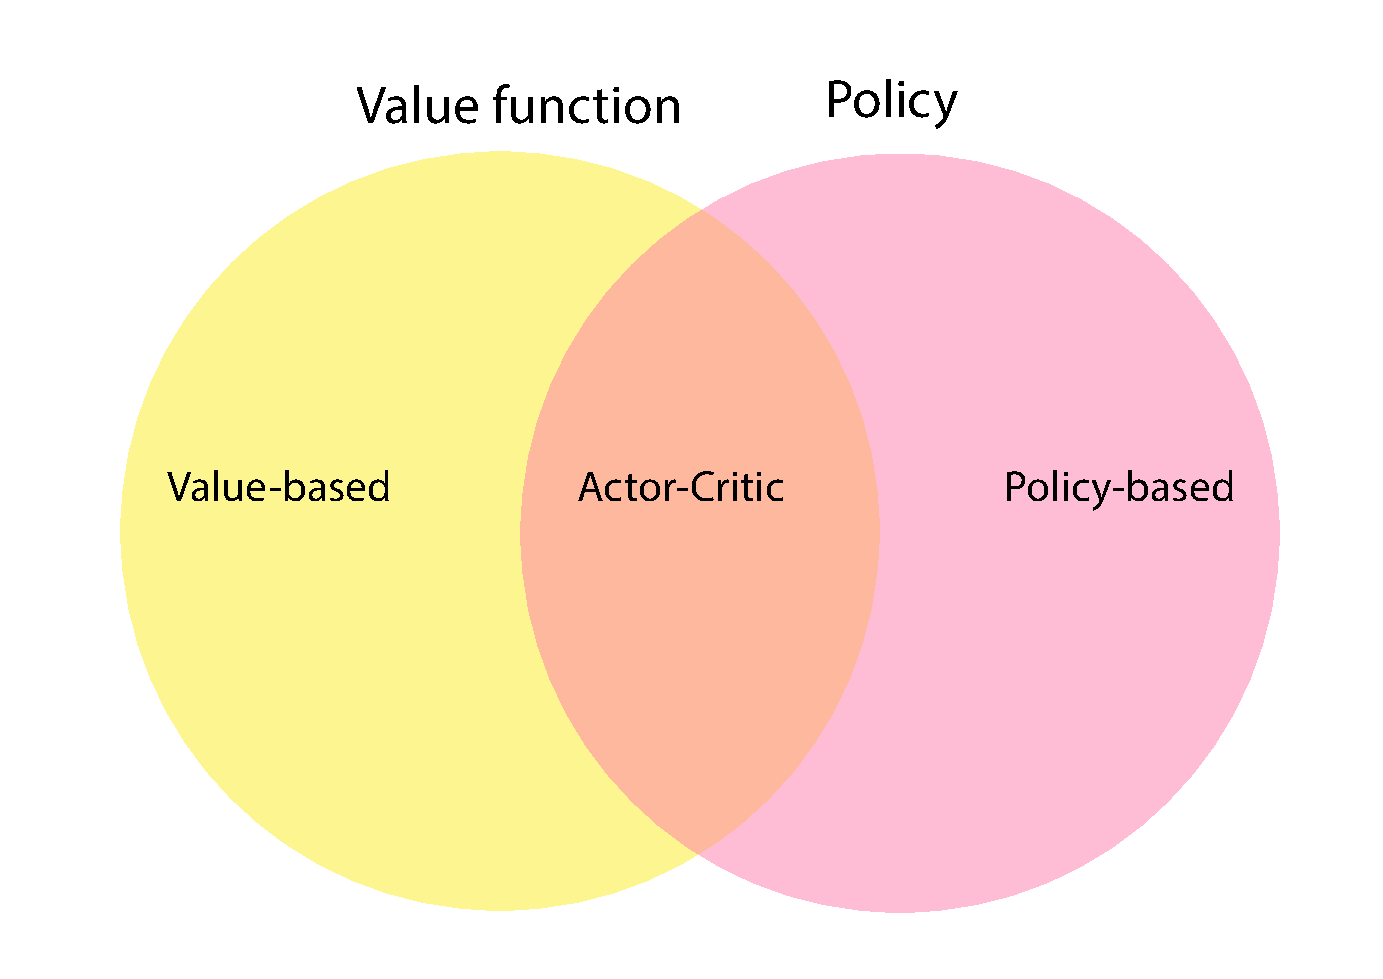
\includegraphics[width=80mm]{figures/valuepolicy.pdf}
\caption{Example of caption}
\label{fig:example}
\end{figure}


\subsection*{Policy based methods}
We parameterize the policy with some unknown parameters $\theta$ 



 
    % end lectures
\end{document}  